% Four ways to spend more computation on one problem at inference time. Values are illustrative.
\documentclass[border=8pt]{standalone}
% Shared TikZ style for every figure in "Post-training LLMs with RL" (see ../STYLE.md).
% Visual grammar follows the FME office-hours house style; the one accent colour is fern green.
% Compile with XeLaTeX, two passes (annotated equations remember node positions).
\usepackage{fontspec}
\setmainfont{Avenir Next}[BoldFont={Avenir Next Demi Bold}, ItalicFont={Avenir Next Italic}]
\setsansfont{Avenir Next}[BoldFont={Avenir Next Demi Bold}, ItalicFont={Avenir Next Italic}]
\renewcommand{\familydefault}{\sfdefault}
\hyphenpenalty=10000 \exhyphenpenalty=10000 % no hyphenation in notes and labels
\usepackage{amsmath,amssymb}
\usepackage{tikz}
\usetikzlibrary{arrows.meta,positioning,calc,fit,backgrounds,shapes.geometric,decorations.pathreplacing}

% ---------------- palette ----------------
\definecolor{ink}{HTML}{111111}
\definecolor{grey700}{HTML}{4A4F55}
\definecolor{grey500}{HTML}{6B7178}
\definecolor{grey400}{HTML}{8A9097}
\definecolor{grey300}{HTML}{D5D9DD}
\definecolor{grey100}{HTML}{F4F5F6}
\definecolor{fern}{HTML}{4F7942}       % the one accent: what the figure is about
\definecolor{ferndark}{HTML}{2F4A28}
\definecolor{fernlight}{HTML}{B5CFA8}
\definecolor{ferntint}{HTML}{EAF1E6}
% aliases used by older figure files
\colorlet{gray7}{grey700}\colorlet{gray5}{grey500}\colorlet{gray3}{grey300}\colorlet{gray1}{grey100}

% ---------------- visual grammar ----------------
\tikzset{
  every picture/.style={line cap=round, line join=round, color=ink},
  tensor/.style={draw=ink, line width=0.8pt, fill=white},
  param/.style={draw=grey700, line width=0.8pt, fill=grey100},
  op/.style={draw=grey500, line width=0.8pt, rounded corners=3pt, fill=white, inner sep=4pt, font=\small},
  accent/.style={draw=fern, line width=1.2pt},
  flow/.style={-{Stealth[length=5pt]}, line width=0.8pt, draw=grey700},
  flowa/.style={flow, draw=fern},
  tname/.style={font=\normalsize, text=ink},
  dims/.style={font=\footnotesize, text=grey500},
  note/.style={font=\footnotesize, text=grey700, align=left},
  accentnote/.style={font=\footnotesize, text=fern, align=left},
  lead/.style={draw=grey400, line width=0.5pt},
  stream/.style={draw=grey300, line width=5pt},
  block/.style={draw=grey500, line width=0.8pt, rounded corners=4pt, fill=white, align=center, font=\small, minimum height=0.8cm},
  blocka/.style={block, accent, fill=ferntint},
  frozen/.style={block, fill=grey100},
  plus/.style={circle, draw=grey700, line width=0.8pt, fill=white, inner sep=0pt, minimum size=0.42cm, font=\small},
  junction/.style={circle, fill=grey700, inner sep=0pt, minimum size=4pt},
  wire/.style={line width=0.8pt, draw=grey700},
}

% ---------------- numbered annotation system ----------------
%   markers on the drawing:  \mk{(x,y)}{1}   \mka{(x,y)}{2} (accent)
%   notes column:            \notesat{(x,y)}{width}  then  \note{1}{text}  /  \notea{2}{text}
%   symbols strip:           \symbols{$x$ & prompt \\ $y$ & response}
\tikzset{
  marker/.style={circle, fill=grey700, text=white, font=\footnotesize\bfseries, inner sep=0pt, minimum size=0.46cm},
  markera/.style={marker, fill=fern},
}
\newcommand{\mk}[2]{\node[marker] at #1 {#2}}
\newcommand{\mka}[2]{\node[markera] at #1 {#2}}
\newlength{\notewidth}
\newcommand{\notesat}[2]{%
  \node[inner sep=0pt, minimum size=0pt, anchor=north west] (note0) at #1 {};
  \setlength{\notewidth}{#2}\xdef\lastnote{note0}}
\newcommand{\note}[2]{%
  \node[font=\small, text=ink, align=left, text width=\notewidth, anchor=north west, inner sep=0pt] (note#1) at ($(\lastnote.south west)+(0.55cm,-0.32cm)$) {#2};
  \node[marker] at ($(note#1.north west)+(-0.30cm,-0.15cm)$) {#1};
  \path (note#1.south west) ++(-0.55cm,0) node[inner sep=0pt, minimum size=0pt] (note#1base) {};
  \xdef\lastnote{note#1base}}
\newcommand{\notea}[2]{%
  \node[font=\small, text=ferndark, align=left, text width=\notewidth, anchor=north west, inner sep=0pt] (note#1) at ($(\lastnote.south west)+(0.55cm,-0.32cm)$) {#2};
  \node[markera] at ($(note#1.north west)+(-0.30cm,-0.15cm)$) {#1};
  \path (note#1.south west) ++(-0.55cm,0) node[inner sep=0pt, minimum size=0pt] (note#1base) {};
  \xdef\lastnote{note#1base}}
\newcommand{\symbols}[1]{%
  \node[anchor=north west, inner sep=0pt, align=left, font=\small, text=grey700] (symbols)
    at ($(\lastnote.south west)+(0,-0.75cm)$)
    {\textcolor{grey400}{\scriptsize\bfseries SYMBOLS}\\[3pt]
     \begin{tabular}{@{}l@{\hspace{8pt}}l@{}}#1\end{tabular}};
  \draw[grey300, line width=0.5pt] ($(symbols.north west)+(0,0.18cm)$) -- ++(\notewidth+0.55cm,0);}

% ---------------- glyphs ----------------
\tikzset{
  expand/.style={draw=grey700, line width=0.8pt, fill=grey100, trapezium, trapezium stretches body,
                 trapezium left angle=64, trapezium right angle=64, shape border rotate=180,
                 minimum height=0.72cm, align=center, font=\small, inner xsep=2pt},
  contract/.style={expand, shape border rotate=0},
  silubox/.style={block, path picture={
      \begin{scope}[sharp corners, shift={($(path picture bounding box.west)+(0.45,-0.05)$)}, x=0.1cm, y=0.1cm]
        \draw[grey300, line width=0.4pt] (-3,0) -- (2.6,0);
        \draw[grey500, line width=1pt, domain=-3:2.4, samples=30] plot (\x, {\x/(1+exp(-\x))});
      \end{scope}}},
}

% ---------------- annotated equations (arrow + plain-language label per term) ----------------
% \tm{name}{math}: wrap one term of a formula in a named node. Put the formula node at (0,0)
% with anchor=base west, otherwise the remembered positions are offset.
\newcommand{\tm}[2]{\tikz[remember picture,baseline=(#1.base)]{\node[inner sep=1pt,outer sep=0pt] (#1) {$\displaystyle #2$};}}
\tikzset{
  lbl/.style   = {font=\large, text=ferndark, align=left, inner sep=2pt},
  lblg/.style  = {lbl, text=grey700},
  arr/.style   = {-{Stealth[length=8pt,width=6pt]}, line width=1.0pt, draw=fern, shorten >=3pt},
  arrg/.style  = {arr, draw=grey500},
  brc/.style   = {decorate, decoration={brace, mirror, amplitude=9pt, raise=5pt}, line width=1.4pt},
  % older diagram styles (kept for existing figures)
  blk/.style   = {draw=grey500, line width=0.9pt, rounded corners=6pt, fill=white, align=center, inner sep=7pt, minimum height=11mm, text=ink},
  blkf/.style  = {blk, draw=fern, line width=1.2pt, fill=ferntint},
  blkg/.style  = {blk, fill=grey100},
  ar/.style    = {-{Stealth[length=7pt,width=5pt]}, line width=1.0pt, draw=grey700},
  arf/.style   = {ar, draw=fern},
  capt/.style  = {font=\normalsize, text=grey500, align=center},
}

% ---------------- annotation protocol for equations ----------------
% The formula is one node named "eq" at (0,0), anchor=base west. Terms are wrapped with \tm.
% Labels sit in fixed rows ABOVE (a) or BELOW (b) the formula, tier 1 (near) or 2 (far), centred on
% their term (optional x-nudge), joined by a straight vertical leader with a dot on the term.
% No curved arrows, no diagonals. Tier-1 labels are at most two lines; tier-2 leaders pass between
% tier-1 labels. Sides l / r (outermost terms only): label beside the term, horizontal leader;
% the 4th argument is then a y-nudge.   \ann{term}{a|b|l|r}{1|2}{nudge}{text}    \anna{...} = accent (the slide's point)
\tikzset{
  annlbl/.style  = {font=\normalsize, text=grey700, align=center, inner sep=1.5pt},
  annlbla/.style = {annlbl, text=ferndark},
  annlead/.style = {draw=grey400, line width=0.6pt},
  annleada/.style= {draw=fern, line width=0.9pt},
}
\newcommand{\annrow}[2]{\ifnum#2=1 #1 0.55cm\else #1 1.95cm\fi}
\newcommand{\anngeneric}[7]{% #1 style-suffix, #2 term, #3 side, #4 tier, #5 nudge, #6 text, #7 lead style
  \if#3a
    \ifnum#4=1 \def\annoff{0.55cm}\else\def\annoff{1.95cm}\fi
    \node[annlbl#1, anchor=south] (ann-#2) at ($(#2.north |- eq.north)+(#5,\annoff)$) {#6};
    \draw[#7] ($(#2.north)+(0,0.13)$) -- (#2.north |- ann-#2.south);
    \fill[#7] ($(#2.north)+(0,0.13)$) circle (1.4pt);
  \else\if#3l
    \node[annlbl#1, anchor=east] (ann-#2) at ($(#2.west)+(-0.6cm,#5)$) {#6};
    \draw[#7] ($(#2.west)+(-0.13,0)$) -- (ann-#2.east |- {$(#2.west)+(0,0)$});
    \fill[#7] ($(#2.west)+(-0.13,0)$) circle (1.4pt);
  \else\if#3r
    \node[annlbl#1, anchor=west] (ann-#2) at ($(#2.east)+(0.6cm,#5)$) {#6};
    \draw[#7] ($(#2.east)+(0.13,0)$) -- (ann-#2.west |- {$(#2.east)+(0,0)$});
    \fill[#7] ($(#2.east)+(0.13,0)$) circle (1.4pt);
  \else
    \ifnum#4=1 \def\annoff{-0.55cm}\else\def\annoff{-1.95cm}\fi
    \node[annlbl#1, anchor=north] (ann-#2) at ($(#2.south |- eq.south)+(#5,\annoff)$) {#6};
    \draw[#7] ($(#2.south)+(0,-0.13)$) -- (#2.south |- ann-#2.north);
    \fill[#7] ($(#2.south)+(0,-0.13)$) circle (1.4pt);
  \fi\fi\fi}
\newcommand{\ann}[5]{\anngeneric{}{#1}{#2}{#3}{#4}{#5}{annlead}}
\newcommand{\anna}[5]{\anngeneric{a}{#1}{#2}{#3}{#4}{#5}{annleada}}

\begin{document}
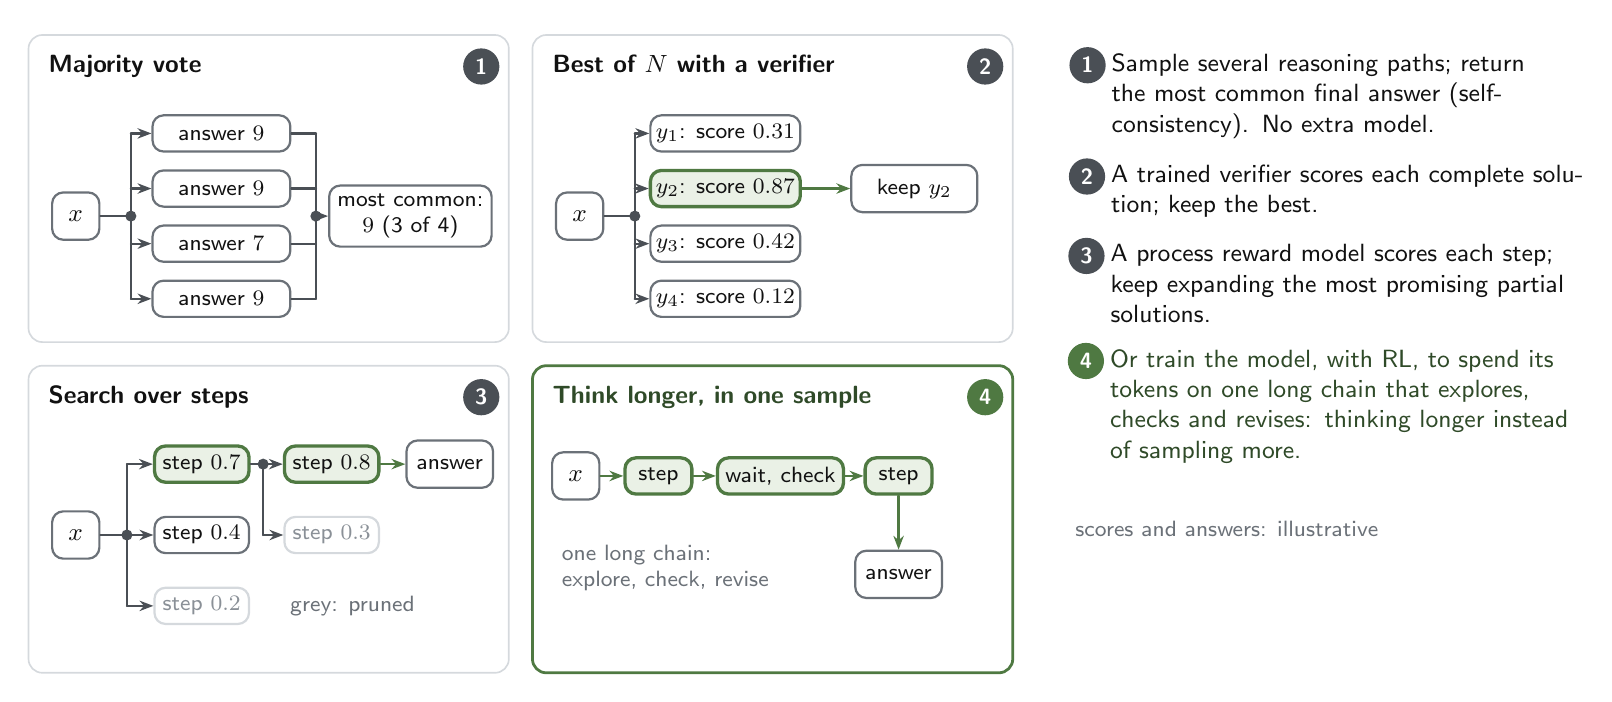
\begin{tikzpicture}[font=\small,
    smp/.style={block, minimum width=1.75cm, minimum height=0.46cm, font=\footnotesize, inner sep=2pt},
    smpa/.style={smp, accent, fill=ferntint},
    smpg/.style={smp, draw=grey300, text=grey400},
    res/.style={block, minimum width=1.6cm, minimum height=0.6cm, font=\footnotesize, align=center, inner sep=3pt},
    xb/.style={block, minimum width=0.6cm, minimum height=0.6cm, font=\small, inner sep=2pt},
    frame/.style={draw=grey300, line width=0.6pt, rounded corners=5pt},
    ptitle/.style={font=\small\bfseries, anchor=north west, inner sep=0}]
  % ---------- panel frames ----------
  \draw[frame] (0,0) rectangle (6.1,-3.9);      \draw[frame] (6.4,0) rectangle (12.5,-3.9);
  \draw[frame] (0,-4.2) rectangle (6.1,-8.1);   \draw[frame, draw=fern, line width=1pt] (6.4,-4.2) rectangle (12.5,-8.1);
  \node[ptitle] at (0.25,-0.25) {Majority vote};
  \node[ptitle] at (6.65,-0.25) {Best of $N$ with a verifier};
  \node[ptitle] at (0.25,-4.45) {Search over steps};
  \node[ptitle, text=ferndark] at (6.65,-4.45) {Think longer, in one sample};
  \mk{(5.75,-0.4)}{1}; \mk{(12.15,-0.4)}{2}; \mk{(5.75,-4.6)}{3}; \mka{(12.15,-4.6)}{4};
  % ---------- 1: majority vote ----------
  \node[xb] (x1) at (0.6,-2.3) {$x$};
  \foreach \i/\a [count=\k] in {1/9, 2/9, 3/7, 4/9} \node[smp] (a\k) at (2.45,{-1.25-0.7*(\k-1)}) {answer $\a$};
  \coordinate (t1) at (1.3,-2.3);
  \draw[wire] (x1.east) -- (t1); \node[junction] at (t1) {};
  \draw[wire] (t1 |- a1.west) -- (t1 |- a4.west);
  \foreach \k in {1,...,4} \draw[flow] (t1 |- a\k.west) -- (a\k.west);
  \coordinate (m1) at (3.65,-2.3);
  \draw[wire] (m1 |- a1.east) -- (m1 |- a4.east);
  \foreach \k in {1,...,4} \draw[wire] (a\k.east) -- (m1 |- a\k.east);
  \node[junction] at (m1) {};
  \node[res] (r1) at (4.85,-2.3) {most common:\\$9$ (3 of 4)};
  \draw[flow] (m1) -- (r1.west);
  % ---------- 2: best of N ----------
  \node[xb] (x2) at (7.0,-2.3) {$x$};
  \foreach \s [count=\k] in {0.31, 0.87, 0.42, 0.12} {
    \ifnum\k=2 \node[smpa] (b\k) at (8.85,{-1.25-0.7*(\k-1)}) {$y_{\k}$: score $\s$};
    \else \node[smp] (b\k) at (8.85,{-1.25-0.7*(\k-1)}) {$y_{\k}$: score $\s$};\fi}
  \coordinate (t2) at (7.7,-2.3);
  \draw[wire] (x2.east) -- (t2); \node[junction] at (t2) {};
  \draw[wire] (t2 |- b1.west) -- (t2 |- b4.west);
  \foreach \k in {1,...,4} \draw[flow] (t2 |- b\k.west) -- (b\k.west);
  \node[res] (r2) at (11.25,-1.95) {keep $y_2$};
  \draw[flowa] (b2.east) -- (b2.east -| r2.west);
  % ---------- 3: search over steps ----------
  \node[xb] (x3) at (0.6,-6.35) {$x$};
  \node[smpa, minimum width=1.2cm] (s11) at (2.2,-5.45) {step $0.7$};
  \node[smp, minimum width=1.2cm]  (s12) at (2.2,-6.35) {step $0.4$};
  \node[smpg, minimum width=1.2cm] (s13) at (2.2,-7.25) {step $0.2$};
  \coordinate (t3) at (1.25,-6.35);
  \draw[wire] (x3.east) -- (t3); \node[junction] at (t3) {};
  \draw[wire] (t3 |- s11.west) -- (t3 |- s13.west);
  \foreach \k in {11,12,13} \draw[flow] (t3 |- s\k.west) -- (s\k.west);
  \node[smpa, minimum width=1.2cm] (s21) at (3.85,-5.45) {step $0.8$};
  \node[smpg, minimum width=1.2cm] (s22) at (3.85,-6.35) {step $0.3$};
  \coordinate (t4) at (2.98,-5.45);
  \draw[wire] (s11.east) -- (t4); \node[junction] at (t4) {};
  \draw[wire] (t4) -- (t4 |- s22.west);
  \draw[flow] (t4) -- (s21.west); \draw[flow] (t4 |- s22.west) -- (s22.west);
  \node[res, minimum width=1.1cm] (r3) at (5.35,-5.45) {answer};
  \draw[flowa] (s21.east) -- (r3.west);
  \node[dims, anchor=west] at (3.2,-7.25) {grey: pruned};
  % ---------- 4: think longer ----------
  \node[xb] (x4) at (6.95,-5.6) {$x$};
  \node[smpa, minimum width=0.85cm] (c1) at (8.0,-5.6) {step};
  \node[smpa, minimum width=1.6cm] (c2) at (9.55,-5.6) {wait, check};
  \node[smpa, minimum width=0.85cm] (c3) at (11.05,-5.6) {step};
  \draw[flowa] (x4) -- (c1); \draw[flowa] (c1) -- (c2); \draw[flowa] (c2) -- (c3);
  \node[res, minimum width=1.1cm] (r4) at (11.05,-6.85) {answer};
  \draw[flowa] (c3) -- (r4);
  \node[dims, anchor=north west, align=left] at (6.65,-6.35) {one long chain:\\explore, check, revise};
  % ---------- notes ----------
  \notesat{(13.2,0.1)}{6.0cm}
  \note{1}{Sample several reasoning paths; return the most common final answer (self-consistency). No extra model.}
  \note{2}{A trained verifier scores each complete solution; keep the best.}
  \note{3}{A process reward model scores each step; keep expanding the most promising partial solutions.}
  \notea{4}{Or train the model, with RL, to spend its tokens on one long chain that explores, checks and revises: thinking longer instead of sampling more.}
  \node[dims, anchor=north west] at ($(\lastnote.south west)+(0,-0.6)$) {scores and answers: illustrative};
\end{tikzpicture}
\end{document}
